% !TEX root = p2-report-real.tex
\documentclass[UTF8,a4paper,zihao=5,fontset=none]{ctexart}
\usepackage[margin=22mm,headheight=15pt,headsep=7mm,footskip=10mm]{geometry}
\usepackage{amsmath,amssymb}
\usepackage{graphicx}
\usepackage{float}
\usepackage{xcolor}
\usepackage{fancyhdr}
\usepackage[unicode,colorlinks=true]{hyperref}

\IfFontExistsTF{SimSun}{
  \setCJKmainfont{SimSun}[BoldFont=SimHei]
  \setCJKsansfont{Microsoft YaHei}
}{
  \IfFontExistsTF{Noto Serif CJK SC}{
    \setCJKmainfont{Noto Serif CJK SC}
    \setCJKsansfont{Noto Sans CJK SC}
  }{
    \setCJKmainfont{FandolSong-Regular}[BoldFont=FandolSong-Bold]
    \setCJKsansfont{FandolHei-Regular}
  }
}
\IfFontExistsTF{Times New Roman}{\setmainfont{Times New Roman}}{\setmainfont{TeX Gyre Termes}}
\definecolor{ink}{HTML}{172326}
\definecolor{muted}{HTML}{627376}
\definecolor{accent}{HTML}{126D70}
\hypersetup{
  pdftitle={文档图像偏色与光照不均：成因、建模与校正},
  pdfsubject={Machine Vision P1},
  pdfauthor={},
  linkcolor=accent,citecolor=accent,urlcolor=accent
}
\color{ink}
\linespread{1.42}
\setlength{\parindent}{2em}
\setlength{\parskip}{0.25em}
\setlength{\emergencystretch}{1em}
\clubpenalty=10000
\widowpenalty=10000
\displaywidowpenalty=10000
\ctexset{
  section={format=\large\bfseries,beforeskip=1em,afterskip=0.5em},
  subsection={format=\normalsize\bfseries,beforeskip=0.8em,afterskip=0.4em}
}
\pagestyle{fancy}
\fancyhf{}
\fancyhead[L]{\small\color{muted}Machine Vision / P1}
\fancyhead[R]{\small\color{muted}文档图像质量技术综述}
\fancyfoot[C]{\small\color{muted}\thepage}
\renewcommand{\headrulewidth}{0.3pt}
\graphicspath{{../figures/}}

\usepackage{booktabs,tabularx,caption}
\IfFontExistsTF{SimSun}{\setCJKmonofont{SimSun}}{\setCJKmonofont{FandolFang-Regular}}
\captionsetup{font=small,labelfont=bf,skip=5pt}
\hypersetup{pdftitle={板书图像多尺度特征匹配质量评测：真实拍摄数据实验},pdfsubject={Machine Vision P2 real textbook photographs}}
\fancyhead[L]{\small\color{muted}Machine Vision / P2}
\fancyhead[R]{\small\color{muted}真实拍摄数据与可重复性消融}
\graphicspath{{../figures/p2-real/}}
\linespread{1.25}
\newcommand{\filepath}[1]{\nolinkurl{#1}}

\begin{document}
\begin{center}
{\LARGE\bfseries 板书图像多尺度特征匹配质量评测}\par
\vspace{3mm}
{\large 可重复性消融实验}\par
\vspace{2mm}
{\small Lab2 / 第 3 周 / 周四 \qquad 2026 年 9 月 18 日}\par
{\small 真实拍摄数据版：教材页面场景}
\end{center}

\begin{abstract}
围绕文字类图像在光照、拍摄尺度和模糊变化下的特征稳定性，建立单一 Python 文件实现的评测流程，比较 Sobel、LoG、Harris、Shi-Tomasi、SIFT 五类匹配管线，结合 FFT 理想/高斯低通、高通预处理及一至三层外部金字塔，统计重复率、匹配正确率、定位误差和运行时间。使用用户提供的十二张同一教材页面的手机照片，一张作参考，其余十一张与参考形成图对；经逐张视觉选点、局部灰度配准辅助和助手放大图核对，共保留二百五十对同名点，每个图对不少于二十对。实验包含三千二百四十五行评测，并绘制尺度、噪声、金字塔深度及三个组件关闭消融的曲线。教材页面不是题目指定的板书或试卷，助手制作的标注也不等同于学生亲手标注，这两项来源边界不作隐瞒。书页弯曲使单应几何参照带有近似误差，结果应联合匹配数量和几何残差解读，而非仅凭一个比例判定可信度。
\end{abstract}

\section{数据、标注与评测范围}
\subsection{真实照片与拍摄变化}
本次输入为 \filepath{IMG_0258.JPG} 至 \filepath{IMG_0269.JPG} 十二张照片，原始尺寸均为 $4284\times5712$。照片反复拍摄同一组书页，包含靠近电脑、过道、柜旁、桌前和强侧拍等视角；可见书页大小、倾斜、明暗与阴影变化，\filepath{IMG_0265.JPG} 和 \filepath{IMG_0268.JPG} 的细节较软。条件标签是从照片内容得到的定性描述，没有测量照度、曝光、焦距、光学模糊参数或真实噪声方差。原生因素同时变化，不能把图间差异独立归因于某一个拍摄因素。

\filepath{IMG_0260.JPG} 为参考图，其余十一张为场景图。全部照片保持宽高比，用 Lanczos 统一缩小为 $960\times1280$，不作透视拉正，也不生成新的拍摄样本。导入时去除 EXIF/GPS 等元数据；原图不改写。清单保存原图文件名、尺寸、SHA-256，以及工作坐标到原图坐标的换算信息。工作坐标原点在左上角，$x$ 向右、$y$ 向下。

\subsection{点对选择、核对及来源声明}
强侧拍使右页表格的部分框线挤压或不可见，因此全部图对统一以左页为主要评测对象。先从原分辨率放大预览逐张选择章标题、下划线、印刷图形、文字标签和项目符号等对应位置，再以局部归一化灰度模板匹配辅助修正坐标。项目符号的行号靠视觉辨认，并仅在初选圆点附近作局部圆心修正，避免重复圆点串行；被测的五类特征检测器不用于生成点对。

助手逐对查看点位中心的放大图，去除裁切、卷曲或难以确认的点。每图保留二十至二十四对，十一图共二百五十对，点号允许不连续。\filepath{IMG_0265.JPG} 的部分下方圆点已在画面外，不强行补出不存在的坐标。标注 JSON 同时保存初选坐标、最终工作坐标、原图等效坐标、标签、局部配准分数及助手复核者；配准分数不是正确匹配概率。

标注状态为 \filepath{assistant_visual_verified}，\filepath{human_verified=false}。这是助手视觉选点、算法辅助与助手核对的标注成果，\textbf{不冒充学生或其他人亲手标注}。数据题材是教材页，\textbf{不是板书或试卷}。十二张真实照片解决了真实图像数量不足的问题，但不据此声称已完全满足作业的题材及人工执行者要求。

\subsection{ROI 与几何参照}
评测 ROI 为每个图对保留标注点的凸包。所有设置在同一图对上共享固定 ROI，特征预算在 ROI 内分配，避免检测结果主要来自桌面、柜子、衣物和键盘。图像本身不清零、不贴掩模背景，频域滤波仍作用于完整工作图像；检测只限制候选点中心，因此描述子邻域可能超出凸包。不同图对的凸包受可见点影响，并不保证完全相同的物理范围。

程序由保留点对拟合场景到参考的单应矩阵 $H$，不使用被测描述子匹配去拟合判分几何。全部点最小二乘拟合，不通过删掉大残差来美化几何质量。另输出重投影 RMSE、最大残差和逐点留一法误差。拟合误差不是独立测试精度；留一法也只检验同一书页标注的几何预测一致性，不能验证检测器泛化。纸面弯曲、局部灰度配准误差和镜头畸变都会使平面模型产生误差。

\begin{figure}[H]
\centering
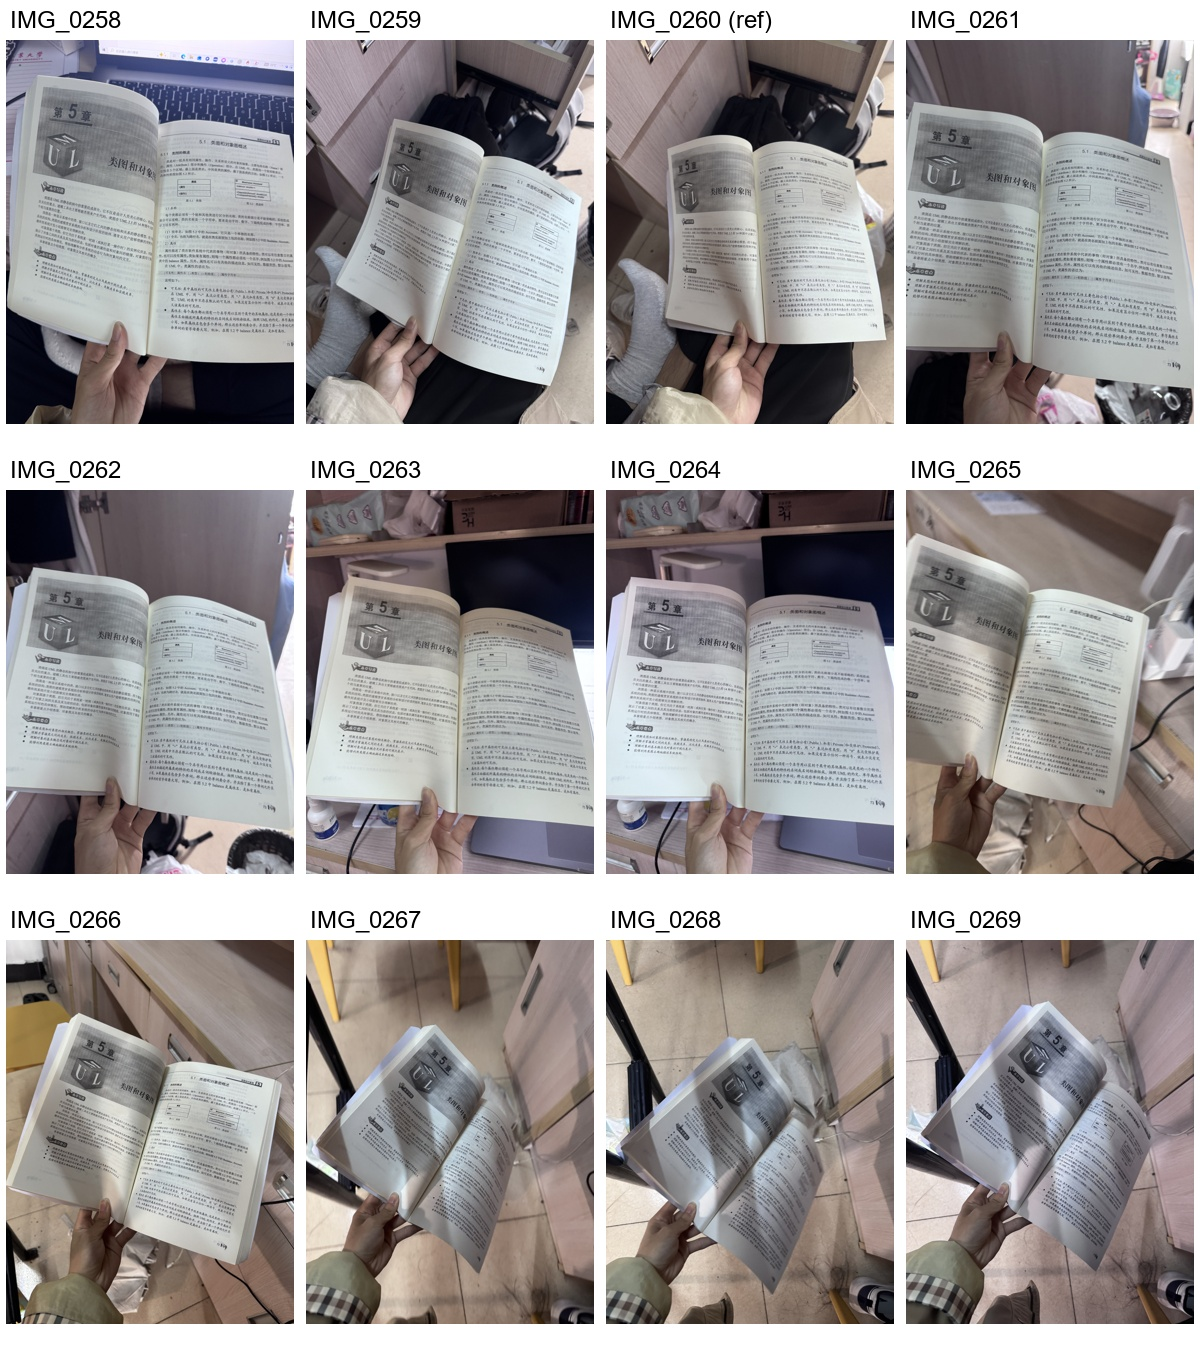
\includegraphics[width=\textwidth,height=0.65\textheight,keepaspectratio]{dataset_contact.jpg}
\caption{同一教材页面在不同拍摄条件下仍保留可对应内容。十二张真实照片的缩略图，文件编号与数据清单一致；这里展示拍摄输入，不是十二份独立原稿。}
\end{figure}

\section{方法与单文件实现}
全部 P2 功能位于 \filepath{p2_multiscale_feature_matching.py}，包括真实照片导入、标注辅助与预览、代理数据生成、校验、特征、匹配、指标、消融、曲线和自检。P1 的实现不参与本次实验，提交包只有一个 Python 文件。

\subsection{空域特征与描述子}
Sobel 在 $3\times3$ 高斯平滑后计算两个方向导数，采样梯度幅值的高响应位置：
\begin{equation}
r_S=\sqrt{I_x^2+I_y^2}.
\end{equation}
LoG 先以 $\sigma=1.2$ 平滑，再计算 $3\times3$ 离散 Laplacian，取绝对响应：
\begin{equation}
r_L=|\nabla^2(G_{1.2}*I)|.
\end{equation}
这里 Sobel 和 LoG 是响应采样点，不声称与角点定义等价；LoG 不使用零交叉或尺度归一化斑点检测。

Harris 与 Shi-Tomasi 使用结构张量及其特征值：
\begin{equation}
M=\sum_W w\begin{bmatrix}I_x^2&I_xI_y\\I_xI_y&I_y^2\end{bmatrix},\qquad
r_H=\det M-0.04(\operatorname{tr}M)^2,\quad r_{ST}=\min(\lambda_1,\lambda_2).
\end{equation}
实现使用 OpenCV \filepath{cornerHarris} 和 \filepath{cornerMinEigenVal}，分别取邻域宽二、三，导数核宽三。保留 Harris 正响应。四种响应采样方法在每层 ROI 中用第九十九百分位阈值；每层独立归一化，固定阈值口径与最终预算。

SIFT 使用 OpenCV 原生尺度空间极值与一百二十八维描述子，参数为 \filepath{contrastThreshold=0.01}、\filepath{edgeThreshold=10}、\filepath{sigma=1.2}。其余四方法取 $32\times32$ 灰度补丁，面积缩放为 $16\times16$，去均值、作 $L_2$ 归一化，得到二百五十六维描述子。因此对比的是完整匹配管线，而不是在共同描述子下纯粹比较检测器。

\subsection{FFT 理想与高斯低通、高通}
以移频后的直流中心计算频率半径 $D$，当前层宽高为 $w,h$：
\begin{align}
F&=\operatorname{fftshift}(\operatorname{FFT2}(I/255)),\\
D(u,v)&=\sqrt{(u-\lfloor w/2\rfloor)^2+(v-\lfloor h/2\rfloor)^2},\\
T_{IL}&=\mathbf 1[D\leq0.12\min(w,h)],\quad T_{IH}=1-T_{IL},\\
T_{GL}&=\exp[-D^2/(2\{0.10\min(w,h)\}^2)],\quad T_{GH}=1-T_{GL},\\
J&=\Re\{\operatorname{IFFT2}[\operatorname{ifftshift}(T\odot F)]\}.
\end{align}
包含不滤波对照，共五种设置。低通输出裁剪至 $[0,1]$；高通按每图百分之一、百分之九十九分位线性映射到八位灰度，因此高通比较还包含对比度归一化。没有 FFT 边界填充，背景和周期边界可能影响 ROI 内响应。这些截止比例是固定实验参数，不是已寻找的最优参数。

\subsection{多尺度与非极大值抑制}
外部金字塔深度 $L=1,2,3$，第 $l$ 层尺度 $2^{-l}$，用面积缩放生成粗层。每层分别滤波与检测，按实际尺寸比例及像素中心约定映回原图：
\begin{equation}
x_0=(x_l+0.5)\frac{w_0}{w_l}-0.5,
\end{equation}
$y$ 同理。融合分数乘 $1/(1+0.2l)$，各层共享最终二百二十点预算。NMS 开启时，四种响应先取 $5\times5$ 局部最大值，再对融合点按分数实施五工作像素的距离抑制；关闭时阈值和预算不变。SIFT 的内部 DoG 极值和尺度空间一直保留，消融只切换共同空间 NMS 和外部金字塔。

\section{指标定义与实验控制}
令 $\pi_H(q)$ 为场景点映到参考的非齐次坐标，误差 $e(p,q)=\|p-\pi_H(q)\|_2$，单位始终为参考工作图像素。先筛除投影不在另一幅图像和其 ROI 内的点，得到共同可见点集 $\mathcal R,\mathcal S$。

按距离升序，在 $e\leq5$ 的候选中贪心保留一对一关系得到 $\mathcal M_r$，定义
\begin{equation}
\mathrm{Rep}=\frac{|\mathcal M_r|}{\min(|\mathcal R|,|\mathcal S|)},\quad
E_{loc}=\operatorname{median}_{\mathcal M_r}e.
\end{equation}
分母为空则重复率为零；没有重复点则定位误差未定义。该口径不是最大基数二分匹配。定位误差是阈值内重复点的条件统计，不是全部检测点或所有标注的误差。

描述子使用 $L_2$ 最近邻，正反方向均通过 $0.78$ 比例检验且互为最近邻，得到接受集 $\mathcal M_a$：
\begin{equation}
\mathrm{Prec}=\frac{\sum_{(p,q)\in\mathcal M_a}\mathbf 1[e(p,q)\leq4]}{|\mathcal M_a|},\quad
t=1000(t_{end}-t_{start})\ \mathrm{ms}.
\end{equation}
无接受匹配时正确率未定义，不按零计算；汇总附有效图对数。时间包含两图预处理、检测、描述、几何筛选及匹配，不含 I/O，单次计时且 OpenCV 单线程。CSV 还保存原始/可见点数、重复点数、接受和正确匹配数及匹配误差。表中的正确率是按近似 $H$ 判断的几何正确率，不是已完成独立像素级或 OCR 语义真值判定。

主矩阵为十一图对、五方法、五预处理和三个深度，共 $825$ 行。完整消融设置为高斯低通、三层、NMS 开启，分别关闭金字塔、频域滤波、NMS，共 $220$ 行。

数字尺度实验固定三层与 NMS，将场景额外缩放到 $0.5,0.75,1,1.25$ 倍，同步变换 ROI 并组合逆 resize 与 $H$，共 $1100$ 行。横轴是数字重采样倍率，不是拍摄距离。噪声实验仅给场景加入标准差 $0,5,10,20$ 灰度级的高斯噪声，共 $1100$ 行；各方法与预处理共用同一标准随机场，随机种子 $20260917$。两项受控后处理是在已有拍摄扰动上继续增加变化，不替代实拍来源。

曲线均值与误差棒按十一图对统计，误差棒是样本标准差，不是置信区间。共享一张参考和同一书页的图对不是十一份独立内容。\filepath{summary.json} 记录参数、版本、平台、线程数、代码及输入哈希；\filepath{verification.json} 记录结果一致性检查。

\clearpage
\section{真实照片结果与几何质量}
\subsection{预处理比较}
表~\ref{tab:real-filters} 固定三层与 NMS，汇总十一图重复率。高斯低通并非所有方法的最优设置：LoG 在该设置下为 $0.749$，Sobel 的高斯高通为 $0.776$，而 SIFT 不滤波为 $0.631$、理想低通为 $0.634$，均高于其高斯低通的 $0.547$。这与印刷字细节、响应类型和描述子不同有关，但单一书页不能支持普遍排名。

\begin{table}[H]
\centering\small
\caption{预处理与管线存在交互。三层、NMS 开启时十一图平均重复率，来自主矩阵三层子集；不是按匹配总数池化的比例。}
\label{tab:real-filters}
\begin{tabular}{lrrrrr}
\toprule
方法 & 不滤波 & 理想低通 & 高斯低通 & 理想高通 & 高斯高通\\
\midrule
Sobel & 0.739 & 0.647 & 0.716 & 0.725 & 0.776\\
LoG & 0.738 & 0.535 & 0.749 & 0.662 & 0.672\\
Harris & 0.686 & 0.520 & 0.709 & 0.684 & 0.664\\
Shi-Tomasi & 0.653 & 0.525 & 0.706 & 0.651 & 0.651\\
SIFT & 0.631 & 0.634 & 0.547 & 0.403 & 0.367\\
\bottomrule
\end{tabular}
\end{table}

\subsection{完整设置：比例不能替代数量}
表~\ref{tab:real-full} 是高斯低通、三层与 NMS 的共同完整设置，不是逐方法挑选最好配置。Sobel 重复率 $0.716$，但每图平均接受匹配只有 $1.91$，正确匹配 $0.73$。SIFT 平均接受 $4.91$、正确 $2.73$，也不能仅凭这些点数保证稳定的几何估计；本实验的 $H$ 是由标注另行拟合，而不是通过这些稀少匹配估计。

此外，SIFT 在不滤波消融中正确率均值为 $0.923$，平均正确匹配 $5.45$，高于完整设置的 $0.541$ 和 $2.73$。该现象说明，对这些处理后的 JPEG，额外高斯低通可能损失 SIFT 所需的细节，不应把“开启滤波”默认等同于更可信。

\begin{table}[H]
\centering\small
\caption{高重复率不保证有足够的正确匹配。完整设置的十一图统计；接受/正确为每图数量均值，有效图对数只针对正确率。无接受匹配的图对不计入正确率均值，但数量均值包含这些图对的零。定位为重复点中位误差的跨图均值，时间为消融阶段单次计时均值。}
\label{tab:real-full}
\setlength{\tabcolsep}{4pt}
\begin{tabular}{lrrrrrr}
\toprule
方法 & 重复率 & 正确率 & 定位/px & 耗时/ms & 接受/正确 & 有效图对\\
\midrule
Sobel & 0.716 & 0.287 & 2.185 & 362.2 & 1.91/0.73 & 9/11\\
LoG & 0.749 & 0.502 & 2.215 & 355.2 & 2.73/1.64 & 9/11\\
Harris & 0.709 & 0.454 & 2.268 & 391.0 & 2.91/1.55 & 6/11\\
Shi-Tomasi & 0.706 & 0.471 & 2.253 & 380.8 & 3.73/2.09 & 8/11\\
SIFT & 0.547 & 0.541 & 2.237 & 803.7 & 4.91/2.73 & 11/11\\
\bottomrule
\end{tabular}
\end{table}

\clearpage
\subsection{标注几何的近似误差}
表~\ref{tab:real-geometry} 将图对的拟合残差单独列出。\filepath{IMG_0258} 与 \filepath{IMG_0269} 的 RMSE 超过五参考工作像素，\filepath{IMG_0265} 超过四像素；书页弯曲与点位误差混合，不能只把这些残差解释成标注错误，也不能忽略它们。较大的留一最大误差说明部分位置存在外推不稳定，按同一平面阈值判分可能出现假阴性。

\begin{table}[H]
\centering\small
\caption{单一平面不能精确描述全部卷曲书页。点数、单应拟合 RMSE 与留一预测误差，单位均为参考工作像素；这些是标注几何一致性，不是检测器的定位误差。}
\label{tab:real-geometry}
\begin{tabular}{lrrrr}
\toprule
场景图 & 点对数 & 拟合 RMSE & 留一中位 & 留一最大\\
\midrule
IMG\_0258 & 23 & 5.54 & 4.27 & 25.79\\
IMG\_0259 & 23 & 1.06 & 0.81 & 4.55\\
IMG\_0261 & 24 & 2.65 & 2.44 & 6.63\\
IMG\_0262 & 24 & 2.75 & 2.22 & 7.32\\
IMG\_0263 & 24 & 2.78 & 2.35 & 7.27\\
IMG\_0264 & 24 & 2.70 & 2.57 & 7.10\\
IMG\_0265 & 20 & 4.59 & 1.89 & 20.67\\
IMG\_0266 & 24 & 2.89 & 2.56 & 7.00\\
IMG\_0267 & 22 & 3.51 & 3.80 & 7.64\\
IMG\_0268 & 20 & 3.43 & 2.18 & 9.46\\
IMG\_0269 & 22 & 5.47 & 3.92 & 26.39\\
\bottomrule
\end{tabular}
\end{table}

\clearpage
\section{组件关闭消融}
关闭外部金字塔的影响并不统一。Sobel、Harris、SIFT 的重复率变化为 $+0.99,+0.50,+3.12$ 个百分点，LoG 和 Shi-Tomasi 为 $-2.32,-0.21$。SIFT 关闭外部金字塔后的正确率提高 $13.55$ 个百分点，但平均正确匹配数从 $2.73$ 变为 $1.45$；比例上升不等于匹配数量更多。

关闭频域滤波时，SIFT 重复率和正确率分别提高 $8.41$、$38.22$ 个百分点。LoG 正确率则下降 $41.83$ 个百分点，平均正确匹配从 $1.64$ 减为 $0.09$。相反方向的变化说明滤波与描述子互相作用；正确率均值的有效图集也不同，表中的差值不是严格同图子集的配对差。

\begin{table}[H]
\centering\small
\caption{关闭不同组件不必然降低全部指标。各关闭设置均值减去完整设置均值，单位为百分点。P、F、N 分别为关闭外部金字塔、频域滤波、共同 NMS；“--”表示关闭后无接受匹配、正确率未定义。最终预算和阈值口径保持固定。}
\label{tab:real-delta}
\setlength{\tabcolsep}{5pt}
\begin{tabular}{lrrrrrr}
\toprule
 & \multicolumn{3}{c}{重复率变化/pp} & \multicolumn{3}{c}{正确率变化/pp}\\
\cmidrule(lr){2-4}\cmidrule(lr){5-7}
方法 & P & F & N & P & F & N\\
\midrule
Sobel & +0.99 & +2.30 & -25.47 & -13.89 & +7.41 & --\\
LoG & -2.32 & -1.12 & -27.77 & -9.05 & -41.83 & --\\
Harris & +0.50 & -2.31 & -11.90 & -17.72 & -45.42 & -45.42\\
Shi-Tomasi & -0.21 & -5.27 & -18.53 & +11.15 & +11.25 & +41.81\\
SIFT & +3.12 & +8.41 & -19.29 & +13.55 & +38.22 & -4.74\\
\bottomrule
\end{tabular}
\end{table}

\clearpage
关闭共同 NMS 后，五种方法重复率均下降。Sobel、LoG 在十一图中都没有通过双向比例检验的接受匹配，不能把其正确率当作零。Shi-Tomasi 的正确率为 $0.889$，但只在三图有接受匹配，每图平均正确数仅 $0.36$，低于完整设置的 $2.09$；其定位误差从 $2.253$ 降到 $1.464$ 像素也只是条件统计改善。重复文字上的近邻候选可能造成描述子相似、比例检验失败；这是与结果相容的解释，而非已独立证明的唯一原因。

\begin{figure}[H]
\centering
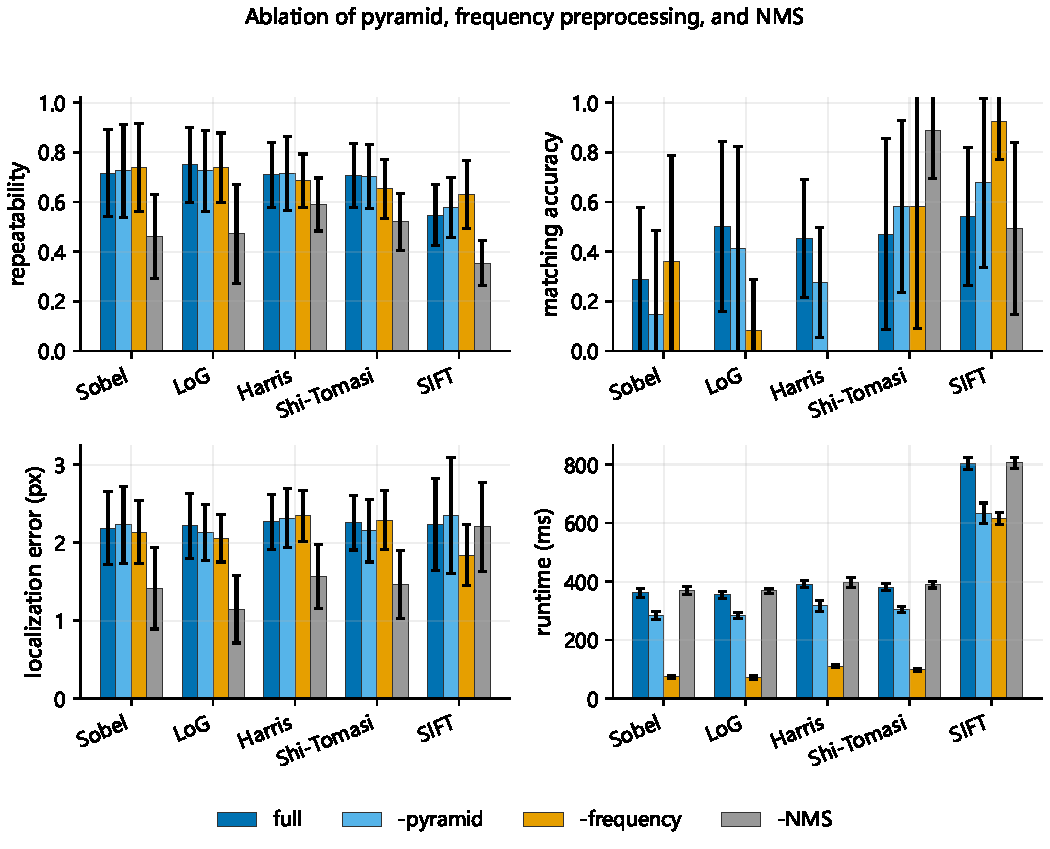
\includegraphics[width=\textwidth]{ablation_metrics.pdf}
\caption{消融需要联合比例、误差和运行时间。四种设置的十一图统计，误差棒为图对之间的样本标准差；正确率面板中未定义的点不绘制，不代表零。接受/正确数量见 CSV，不能只看该图中的比例。}
\end{figure}

\clearpage
\section{多尺度与噪声敏感性}
\subsection{外部金字塔深度}
三层设置并非普遍优于单层。下图的横轴是外部深度而非物理拍摄尺度；每个面板保持一种频域设置，五种管线以颜色、标记及线型共同区分。粗层去噪、细节损失与候选预算竞争同时存在，增加深度的变化应按实际曲线解读。
\begin{figure}[H]
\centering
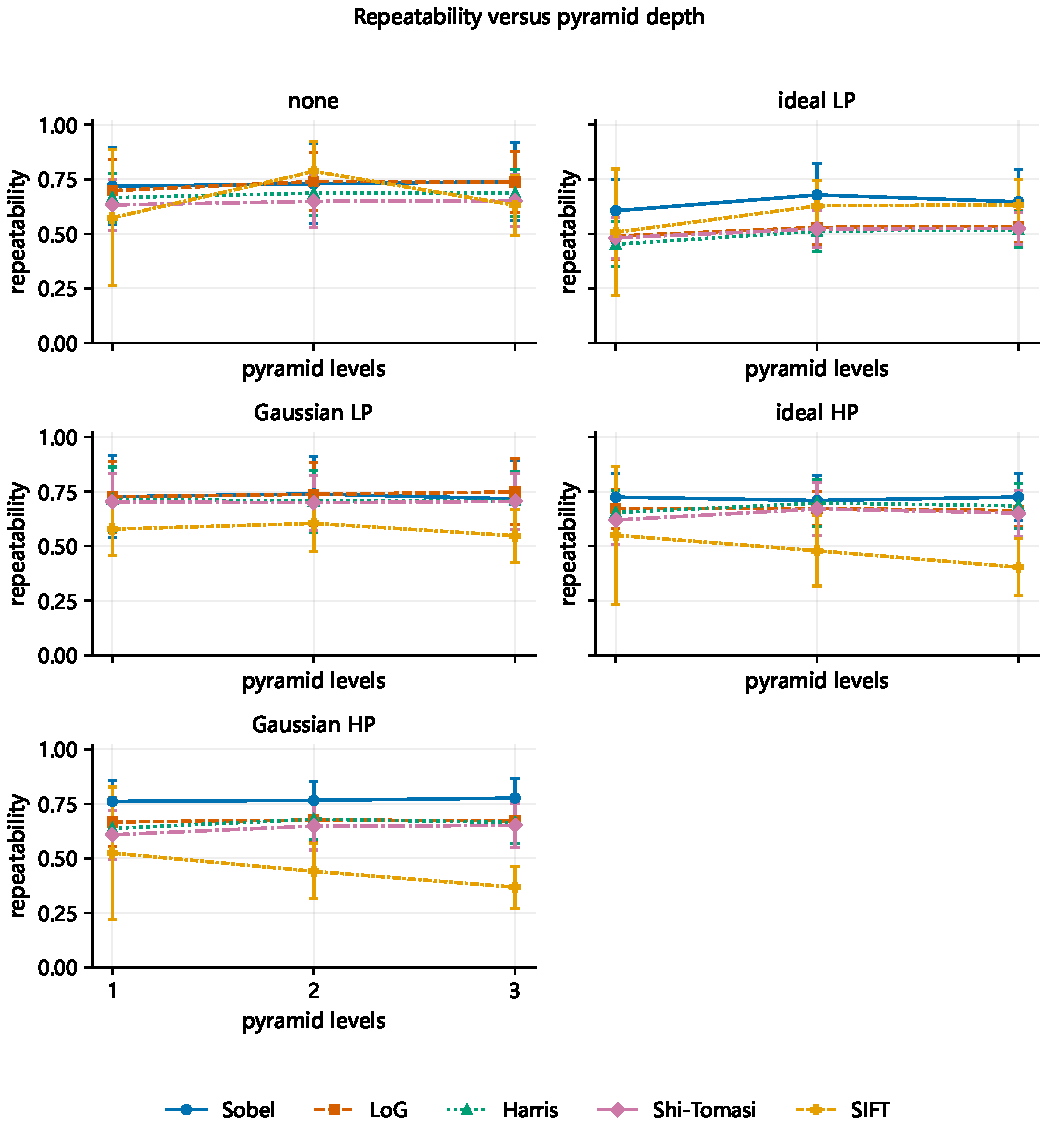
\includegraphics[width=\textwidth,height=0.72\textheight,keepaspectratio]{repeatability_pyramid.pdf}
\caption{外部层数的增加对各管线并非统一收益。深度一至三层、每层分别预处理，最终总预算固定二百二十；LP、HP 表示低通、高通，误差棒为十一图对样本标准差。SIFT 内部尺度空间始终开启。}
\end{figure}

\clearpage
\subsection{受控数字尺度}
下图只改变场景工作图的重采样倍率，参考不变，几何和 ROI 同步换算，误差仍按参考工作像素计。它补充了原生远近拍摄变化，但不等价于改变焦距、真实光学成像或获得新的独立照片。

不滤波时，LoG 在四个倍率下的重复率依次为 $0.538,0.640,0.738,0.750$，缩小后细节损失较明显；Sobel 为 $0.711,0.680,0.739,0.796$，并非严格单调。SIFT 为 $0.548,0.679,0.631,0.601$，在 $0.75$ 倍处最高，不能将数字放大解释为普遍提高尺度稳定性。上述变化同时包含重采样、候选点数量、固定预算与几何判分的影响。
\begin{figure}[H]
\centering
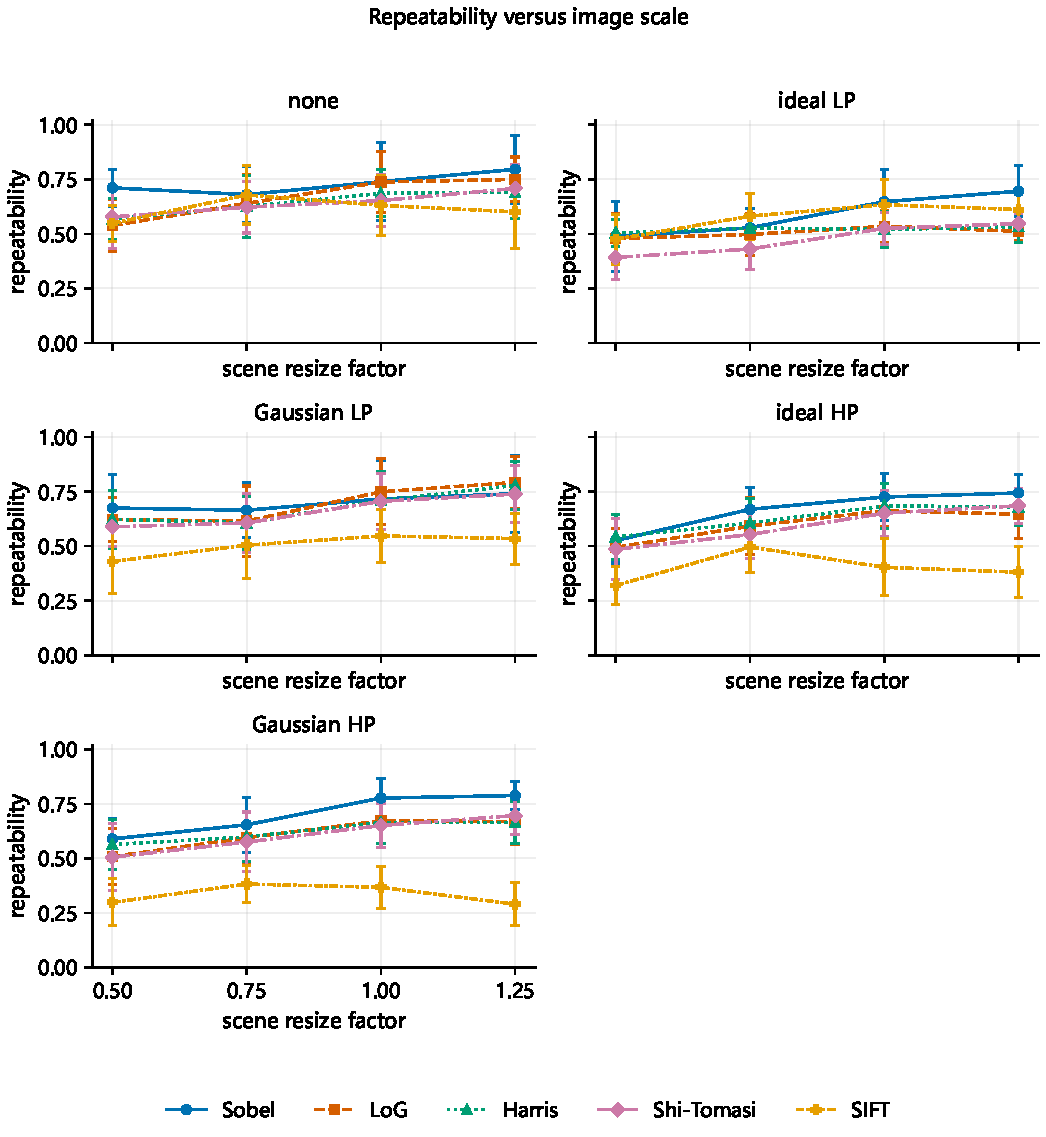
\includegraphics[width=\textwidth,height=0.72\textheight,keepaspectratio]{repeatability_scale.pdf}
\caption{数字重采样检验的是现有 JPEG 管线的尺度敏感性。场景倍率为 $0.5,0.75,1,1.25$，三层、NMS 开启，五预处理分别成面板；横轴不是金字塔层数，误差棒为十一图对样本标准差。}
\end{figure}

\clearpage
\subsection{受控附加噪声}
在高斯低通下，Sobel 的重复率从附加噪声标准差零时的 $0.716$ 变为二十时的 $0.681$，SIFT 从 $0.547$ 变为 $0.481$。Harris 则约为 $0.709$ 到 $0.710$，LoG 中间噪声强度还出现轻微上升。不能据此断言后两种方法对噪声完全不敏感：密集响应点的几何接近、固定预算和近似 $H$ 都影响这个比例，重复率也不衡量描述子是否正确匹配。
\begin{figure}[H]
\centering
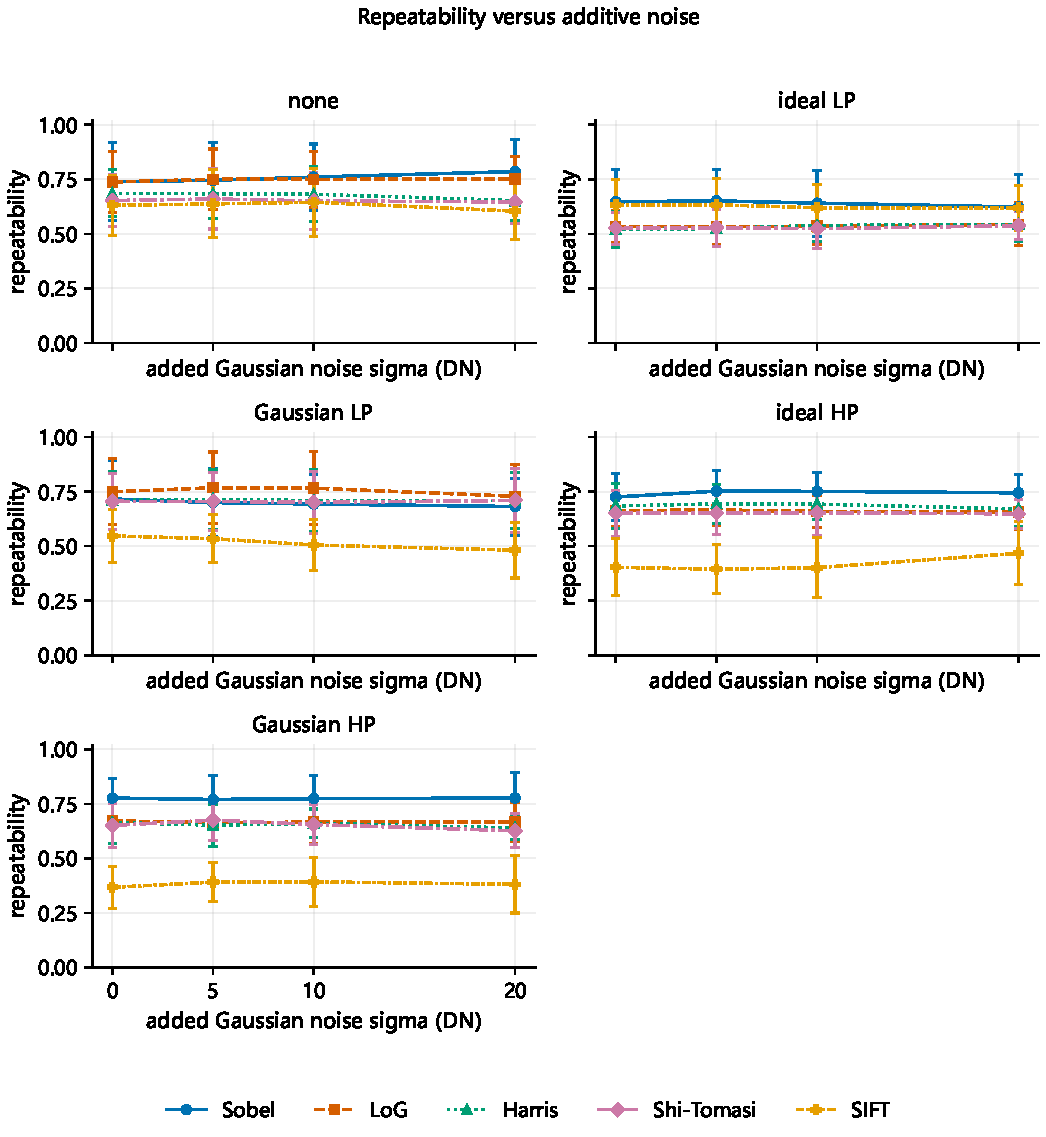
\includegraphics[width=\textwidth,height=0.72\textheight,keepaspectratio]{repeatability_noise.pdf}
\caption{噪声曲线并非全部单调，单一重复率不足以证明可靠性。仅场景额外加入高斯噪声，标准差为 $0,5,10,20$ 灰度级，已有拍摄扰动保留；三层、NMS 开启，误差棒为十一图对样本标准差。}
\end{figure}


\clearpage
\section{计算摄影链路与匹配可信度}
从内容与照明、光学与运动、传感器采样和 ISP，到频域/多尺度预处理、描述子及几何判分，任一环节都能改变末端匹配。此次数据是手机处理后的 JPEG，已经包含未标定的曝光、压缩、去噪和锐化；没有采集 RAW 或测量 ISP。后处理消融说明的是当前管线的敏感性，不独立证明成像物理因果关系。

照明变化往往较平缓，而笔画与边缘含较高频成分，但噪声与细节并不严格分频。低通可能减少噪声，同时抹去小字和角点；高通可能减弱缓变亮度，却也会增强噪声、改变灰度描述子。理想突变截止可能产生振铃，高斯传递函数较平滑，但本实验没有独立量化振铃幅度，因此只把它作为机制解释，而非已测量收益。

粗层扩大有效支持域并平均局部扰动，也会丢失细笔画。固定总预算下，粗层候选可能挤占原图稳定点；对 SIFT，外部金字塔还与内部尺度空间叠加，所以更多层不保证重复率或正确率一起提高。尺度融合的分数归一化和层权重同样影响结果，不能把一种融合策略的表现推广为所有多尺度方法。

NMS 减少同一笔画附近的重复响应，有助于覆盖和描述子唯一性。关闭 NMS 即使得到更小的条件定位误差或更高的正确率，也可能只剩很少接受匹配。匹配可信度应联合重复点、接受/正确数量、覆盖、误差和时间判断。正确率不是单个匹配的概率校准值；共享近似单应矩阵也使几何误差影响多个指标。

\section{局限、结论与复现}
该数据只有一份教材内容，且灰色背景、印刷文字和卷曲纸面不同于白底试卷或真实板书。标注由助手制作并复核，不具备学生亲手标注的来源证明。教材题材和执行者这两项与作业字面要求的偏差已明确保留，不能只改状态字段就宣称完全合规。

单应矩阵是近似几何：部分图对的标注拟合残差接近或大于四/五像素判分阈值，正确的视觉对应也可能被判成不正确，低重复率不一定完全源于检测器。局部模板配准对文字重复、阴影和模糊也存在不确定性；放大核对能减少明显错误，不等于独立人工真值。不同描述子、贪心配对、单次计时及未测试多个独立原稿限制了结论范围。

本次交付包括十二张工作照片、十一份逐图标注、单文件实现、主矩阵、三个组件关闭消融、尺度与噪声曲线、逐图 CSV、运行环境和哈希记录，以及配套报告。结果回答的是这些实拍教材页面在固定预算和几何口径下的匹配敏感性，不宣称某一方法普遍最好。频域与多尺度的价值需要按完整计算摄影链路判断，并结合匹配数量和几何参照的不确定性。

在提交包或仓库根目录运行（PowerShell 每条写成一行）：
\begin{verbatim}
python -m pip install -r requirements-p2.txt
python p2_multiscale_feature_matching.py --self-test
python p2_multiscale_feature_matching.py
  --data-root data/private/p2 --validate-only
python p2_multiscale_feature_matching.py
  --data-root data/private/p2
  --output-root output/p2-real --figure-root figures/p2-real
\end{verbatim}
上述分行仅用于排版，实际命令见 \filepath{P2_REAL_README.md}。已有工作照片与最终 JSON 是复现优先输入。重新运行不会自动修改 PDF 数字，复核时优先对照逐图 CSV、汇总和文件哈希；时间受硬件负载影响。严格人工模式 \filepath{--require-manual} 会拒绝当前助手标注，这是来源约束的预期行为。

\clearpage
\begin{thebibliography}{9}
\small
\bibitem{opencvfeatures} OpenCV contributors. Feature Detection and Description. OpenCV 4.x 官方教程。\url{https://docs.opencv.org/4.x/db/d27/tutorial_py_table_of_contents_feature2d.html}。
\bibitem{opencvgradients} OpenCV contributors. Image Gradients. OpenCV 4.x 官方教程。\url{https://docs.opencv.org/4.x/d5/d0f/tutorial_py_gradients.html}。
\bibitem{opencvfft} OpenCV contributors. Fourier Transform. OpenCV 4.x 官方教程。\url{https://docs.opencv.org/4.x/de/dbc/tutorial_py_fourier_transform.html}。
\end{thebibliography}
\end{document}
